\documentclass{beamer}
%
% Choose how your presentation looks.
%
% For more themes, color themes and font themes, see:
% http://deic.uab.es/~iblanes/beamer_gallery/index_by_theme.html
%
\mode<presentation>
{
  \usetheme{Boadilla}      % or try Darmstadt, Madrid, Warsaw, ...
  \usecolortheme{dove} % or try albatross, beaver, crane, ...
  \usefonttheme{default}  % or try serif, structurebold, ...
  \setbeamertemplate{navigation symbols}{}
  \setbeamertemplate{caption}[numbered]
} 

\usepackage[english]{babel}
\usepackage[utf8x]{inputenc}
\usepackage{booktabs}
\usepackage{appendixnumberbeamer }
\usepackage{multirow}
\usepackage{bigstrut}
\usepackage[justification=centering]{caption}
\usepackage{setspace}
\usepackage{indentfirst}
\usepackage{tabulary}
\usepackage{prettyref}
\usepackage[flushleft]{threeparttable}
\usepackage{tikz}
\def\checkmark{\tikz\fill[scale=0.4](0,.35) -- (.25,0) -- (1,.7) -- (.25,.15) -- cycle;}
\setbeamertemplate{itemize items}[default]
\setbeamertemplate{enumerate items}[default]

\title[Big Questions]{Answering the Big Questions \\ New Information in the 2016 Elections}
\author[Adam Olson]{Adam Olson}
%\institute[UMN]{University of Minnesota, Twin Cities}
\date{September 13th, 2016}

\begin{document}
\begin{frame}
	\titlepage
\end{frame}
\begin{frame}{Plan of the Day}
\tableofcontents
\end{frame}
\section{Importance of Campaigns}
\begin{frame}{Importance of Campaigns}
Generally we think that if campaigns are more or less equal then their effect is more subtle.\\
\medskip
The consequence is that the ins and outs of campaigns are less important than you think.
\end{frame}
\begin{frame}{Importance of Campaigns}
\begin{center}
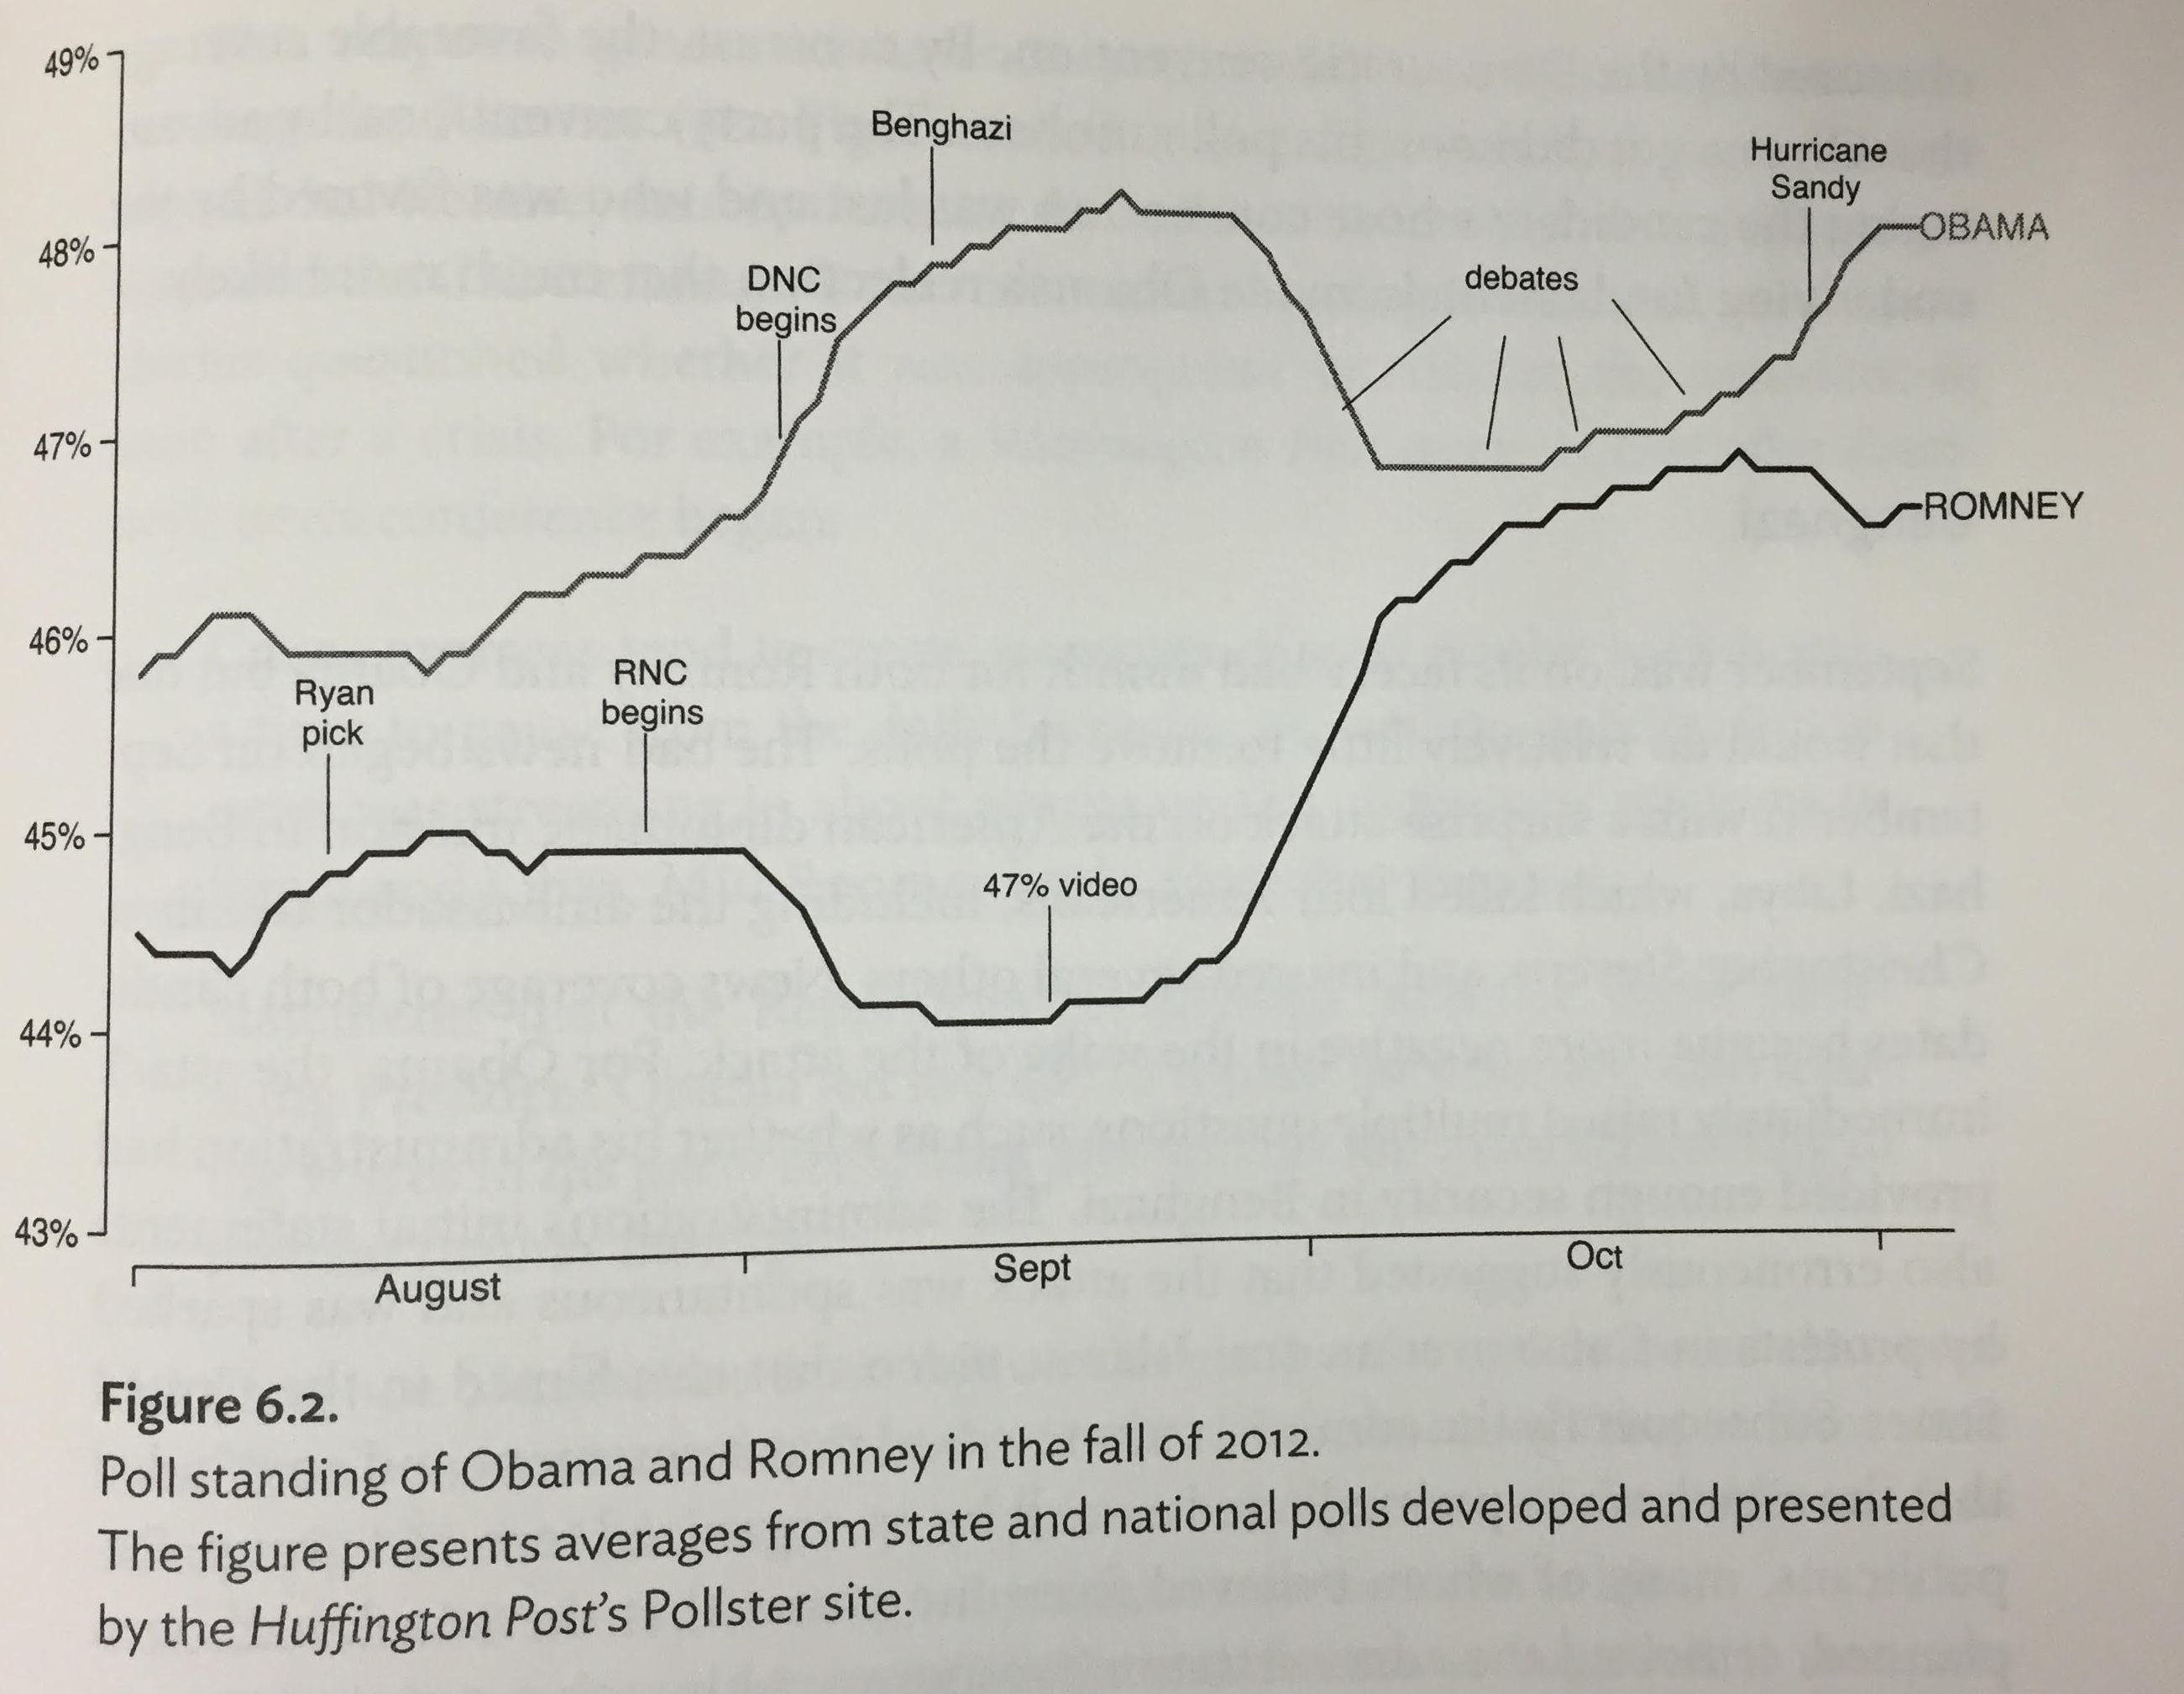
\includegraphics[width=.9\textwidth]{gaffes}
\end{center}
\end{frame}
\begin{frame}{Importance of Campaigns}
One of the largest things a campaign can do is turn out partisans to vote and [decrease/increase] the salience of the economy.
\end{frame}
\begin{frame}{Importance of Independents}
\begin{table}
\centering
\begin{threeparttable}
\caption*{Distribution of Partisans Over Time}
\begin{tabular}{lcccccccccc}\toprule
	&	'90	&	'92	&	'94	&	'96	&	'98	&	'00	&	'02	&	'04	&	'08	&	'12	\\ \midrule
DEM	&	52	&	50	&	47	&	52	&	51	&	50	&	49	&	50	&	51	&	46	\\
IND	&	12	&	13	&	11	&	10	&	12	&	13	&	7	&	10	&	11	&	14	\\
GOP	&	36	&	37	&	41	&	38	&	37	&	37	&	43	&	41	&	37	&	39	\\ \bottomrule
\end{tabular}
\begin{tablenotes}
\tiny
\item This is the measurement of partisans in the United States as measured by the American National Election Study. The original question asks if people lean one way or another and this lumps leaners into their relevant partisan group.
\end{tablenotes}
\end{threeparttable}
\end{table}
\end{frame}

\begin{frame}{Presidential Defections}
\begin{table}
\centering
\begin{threeparttable}
\caption*{Defection Rates in Presidential Voting}
\begin{tabular}{lcccccccccc}\toprule
	&	76	&	80	&	84	&	88	&	92	&	96	&	00	&	'04	&	'08	\\ \midrule
Dem Voting GOP	&	19	&	26	&	21	&	15	&	9	&	6	&	11	&	9	&	9	\\
GOP Voting Dem	&	14	&	7	&	5	&	10	&	12	&	16	&	10	&	8	&	10	\\
Total Not Voting Party ID	&	16	&	24	&	13	&	12	&	24	&	16	&	12	&	10	&	9	\\ \bottomrule
\end{tabular}
\begin{tablenotes}
\tiny
\item The original question asks if people lean one way or another and this lumps leaners into their relevant partisan group. The higher rate of percentages among the total are because of Anderson in 1980 and Perot in 1992.
\end{tablenotes}
\end{threeparttable}
\end{table}
\end{frame}
\section{Popularity of Candidates}
\begin{frame}{Popularity of Candidates}
\begin{center}
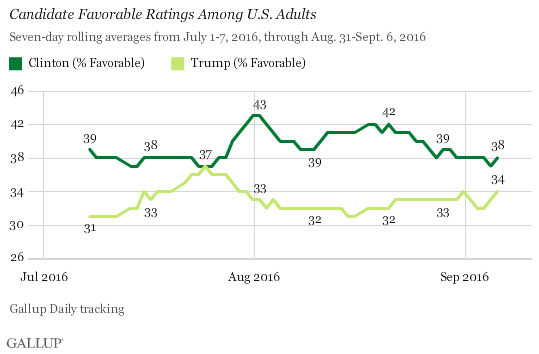
\includegraphics[width=.9\textwidth]{popularity}
\end{center}
\end{frame}
\begin{frame}{Popularity of Candidates Among Partisans}
\begin{table}
\centering
\begin{threeparttable}
\caption*{Support of Candidates Over Time Among Relevant Partisan}
\begin{tabular}{lccc}\toprule
	&	April	&	July	&	September	\\	\midrule
Trump	&	52	&	69	&	74	\\		
Clinton	&	66	&	77	&	79	\\	\bottomrule
\end{tabular}
\begin{tablenotes}
\tiny
\item This is taken from the Gallup Daily Tracking Poll for an arbitrary day in each month. September was collected Aug. 31-Sept. 6, 2016, July was collected around the 15th and April was collected around the 15th as well
\end{tablenotes}
\end{threeparttable}
\end{table}

\end{frame}
\section{Trumpism}
\begin{frame}{What Explains Trump Support}
By far the biggest thing I hear is `how could this be happening' with respect to Donald Trump earning the Republican Nomination
\end{frame}
\begin{frame}{Racial Resentment}
Political Science has mostly focused on three individual level predictors of Trump Support.
\begin{itemize}
\item Populism
\item Authoritarianism
\item \textbf{Racial Resentment}
\end{itemize}
\end{frame}
\begin{frame}{Racial Resentment}
Racial Resentment, as we measure it, is four questions grouped together. It predicts a ton of stuff.
\begin{itemize}
\item It is the second biggest predictor of Obama approval to partisan identification
\item Biggest predictor of disliking welfare
\end{itemize}
\end{frame}
\begin{frame}{Emerging Study}
Racial Resentment is the biggest predictor of support for Trump.
\end{frame}
\begin{frame}{Emerging Study}
``Moving from the least to the most resentful view of African Americans \textbf{increases support for Trump by 44 points}, those who think \textbf{Obama is a Muslim (54 percent of all Republicans) are 24 points more favorable to Trump}, and those who think the word `\textbf{`violent'' describes Muslims extremely well are about 13 points more pro-Trump} than those who think it doesn’t describe them well at all.''

\end{frame}
\section{Wrapping Up}
\begin{frame}{Wrapping Up}
Those are what I think are some of the important things you should keep in mind as election season starts up in earnest.\\
\medskip
e-mail: \texttt{olso4075@umn.edu} \\
website: adamolson.org
\end{frame}
\appendix
\begin{frame}{Racial Resentment Questions}
The racial resentment scale is produced by pooling answers of four questions.
\begin{enumerate}
\item Over the past few years, blacks have gotten less than they deserve. 
\item Irish, Italian, Jewish, and many other minorities overcame prejudice and worked their way up. Blacks should do the same without any special favors.
\item It's really a matter of some people not trying hard enough; if blacks would only try harder they could be just as well off as whites.
\item Generations of slavery and discrimination have created conditions that make it difficult for blacks to work their way out of the lower class.
\end{enumerate}
\end{frame}
\begin{frame}{Regression Coefficients}
\begin{center}
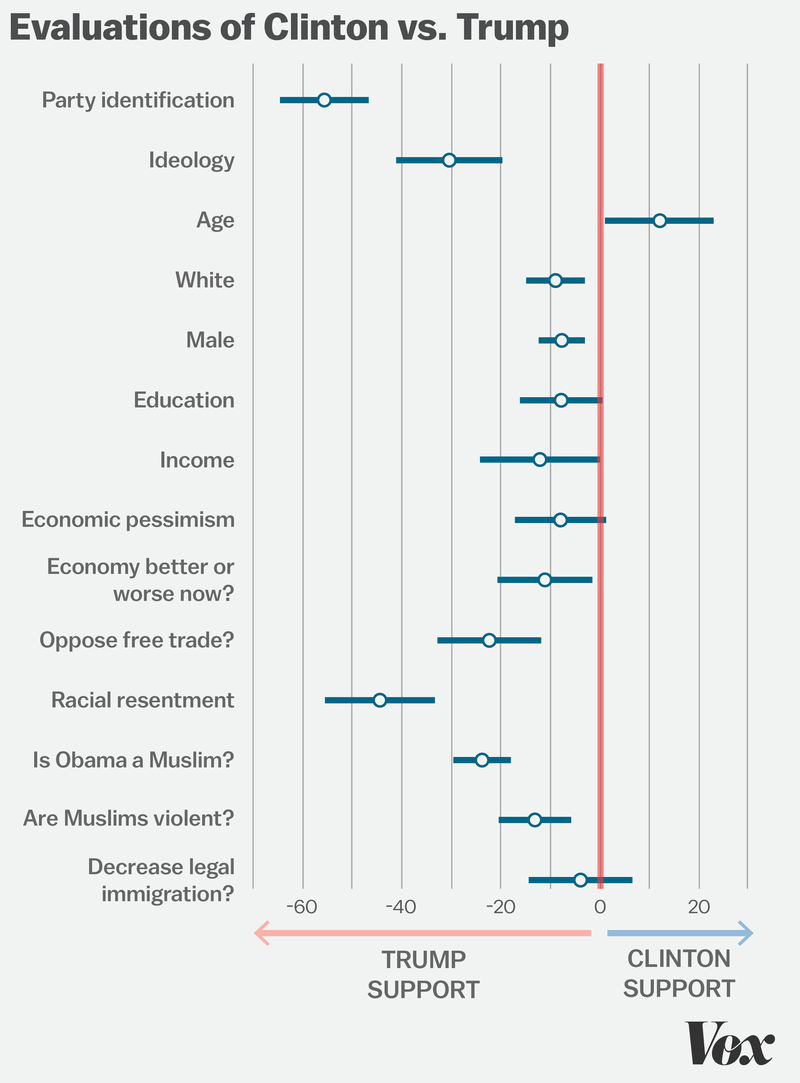
\includegraphics[width=.5\textwidth]{predictors}
\end{center}
\end{frame}
\end{document}